\documentclass[english,11pt,a4paper]{article}
\usepackage[T1]{fontenc} % --------------| More characters.
\usepackage[utf8]{inputenc} % -----------| Direct use of scandinavian letters.
\usepackage{float} % --------------------| More options for floats.
\usepackage{graphicx} % -----------------| Support more image formats.
\usepackage{booktabs} % -----------------| Better-looking tables.
\usepackage{tabularx} % -----------------| Better tables
\usepackage{subcaption} % ---------------| Subfigures.
\usepackage[a4paper]{geometry} % --------| Adjusting page margins.
\usepackage{amsmath,amssymb,amsfonts} % -| Various math, including eqref.
\usepackage{xcolor} % -------------------| Allows defn. of custom colors.
\usepackage{babel}
\usepackage{url}
\usepackage{enumitem}

% XY-pic. Used for creating illustrations.
\input xy
\xyoption{all}

% Styling captions.
\usepackage{caption}
\captionsetup{margin=10pt,font=small,labelfont=bf}


%******************************************************************************
% Includes the listings package and sets some settings for it.
% REQUIRES the `color' package.
%******************************************************************************

\usepackage{listings} % -----------------------| Used for source code listings.
\definecolor{lst-gray}{RGB}{100,100,100}  % ---|Color for line-numbers.
\definecolor{lst-light-gray}{RGB}{250,250,250} % Background color for listings.
\lstset{
  aboveskip=0em, % -------------------| Skip above listing box.
  backgroundcolor=\color{lst-light-gray}, % Background color.
  basicstyle=\ttfamily\scriptsize, % -| Default font style.
  belowskip=\topskip, % --------------| Skip below listing box.
  breakatwhitespace=false, % ---------| Automatic breaks only at whitespace?.
  breaklines=true, % -----------------| Sets automatic line breaking.
  captionpos=t, % --------------------| Sets the caption-position to bottom.
  commentstyle=\color{green}, % ------| Comment style.
  escapeinside={\%*}{*)}, % ----------| For adding LaTeX within code.
  frame=single, % --------------------| Adds a frame around the code.
  keepspaces=true, % -----------------| Keeps spaces in text.
  keywordstyle=\color{blue}, %--------| Keyword style.
  language={C}, % --------------------| The language of the code.
  literate={æ}{{\ae}}1 % -------------| Character conversions
           {Æ}{{\AE}}1
           {ø}{{\oe}}1
           {Ø}{{\OE}}1
           {å}{{\aa}}1
           {Å}{{\AA}}1
           {µ}{{\ensuremath{\mu}}}1,
  numbers=left, % --------------------| Line-number position: none/left/right.
  numbersep=5pt, % -------------------| Distance between line-numbers and code.
  numberstyle=\tiny\color{lst-gray}, %| The style that used for line-numbers.
  rulecolor=\color{black}, % ---------| Frame color.
  showspaces=false, % ----------------| Show spaces with underscores.
  showstringspaces=false, % ----------| Underline spaces within strings.
  showtabs=false, % ------------------| Show tabs with underscores.
  stepnumber=2, %---------------------| Step between two line-numbers..
  stringstyle=\color{red}, % ---------| String literal style.
  tabsize=4, % -----------------------| Sets default tabsize to 2 spaces.
  title=\lstname % -------------------| Show the filename of included file.
}

\begin{document}
\title{Reservoir Simulation, Exercise 3}
\author{Einar Baumann}
\maketitle
\thispagestyle{empty}

\section{Data and plots} % (fold)
\label{sec:data_and_plots}

All plots are shown in in the following pages. Only plots showing \emph{both} lines for DRSDT=0 and the default DRSDT setting are shown.

The DATA file was modified to include the gas-oil ratio and BHP for the injection well by inserting the following lines in the summary section:
\begin{verbatim}
-- WELL GAS-OIL RATIO FOR INJECTOR
WGOR
'INJECTOR'
/
-- WELL BOTTOM-HOLE PRESSURE
WBHP
'INJECTOR'
/
\end{verbatim}

\noindent This is why I've named the plotted data ``...\_mod''. The lines labeled ``...\_mod\_6'' are the lines from assignment 6, i.e. with DRSDT defaulted. These are in all cases the red lines. Views of water, oil and gas saturation in the uppermost block layer ($z=1$) are shown on the last three pages.
% section data_and_plots (end)

\section{DRSDT: Maximum rate of increase of solution GOR} % (fold)
\label{sec:drsdt_maximum_rate_of_increase_of_solution_gor}

% section drsdt_maximum_rate_of_increase_of_solution_gor (end)
When DRSDT is set to 0, which it initially is in the file and thus on the black lines in the plots, the solution GOR is not allowed to rise; i.e. none of the injected (or reservoir) gas is dissolved into the reservoir oil, even if it is undersaturated. When it is defaulted the re-solution rate is unrestricted (equivalent to DRSDT=inf), and $R_s$ will rise very quickly until there is either no free gas left or the oil is saturated.

In graphs with DRSDT=0 we observe at around 09/84 a sudden drop in WBHP at the producer, accompanied by a sudden rise in WGOR. This is caused by the reservoir hitting the bubble point pressure, releasing the solution gas.

The same behaviour probably occurs for the DRSDT=inf graph at a later point (outside the simulated time span). This likely has something to do with the oil swelling due to the absorbed injection gas.


\pagebreak
\centerline{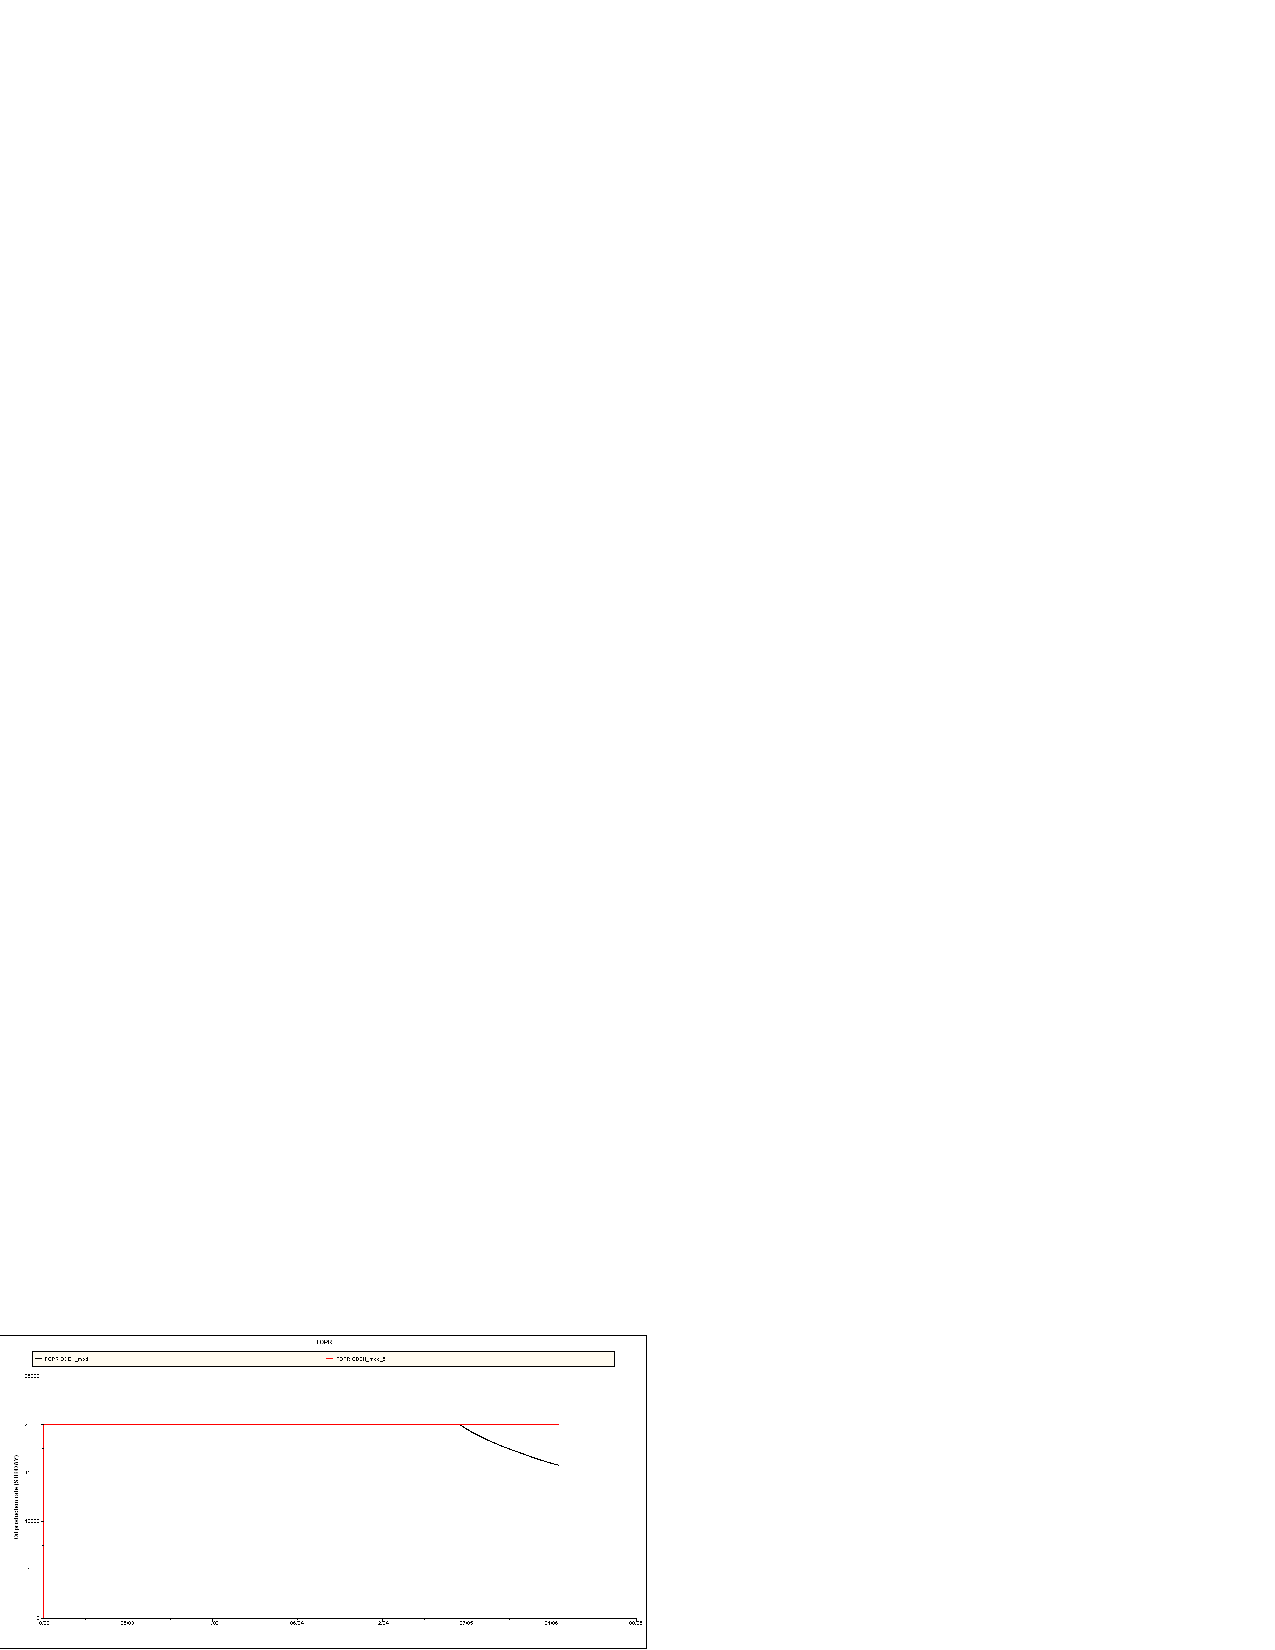
\includegraphics[clip=true, trim=0cm 0cm 10.6cm 22.6cm,width=1.3\textwidth]{graphics/fopr_comb.pdf}}
\centerline{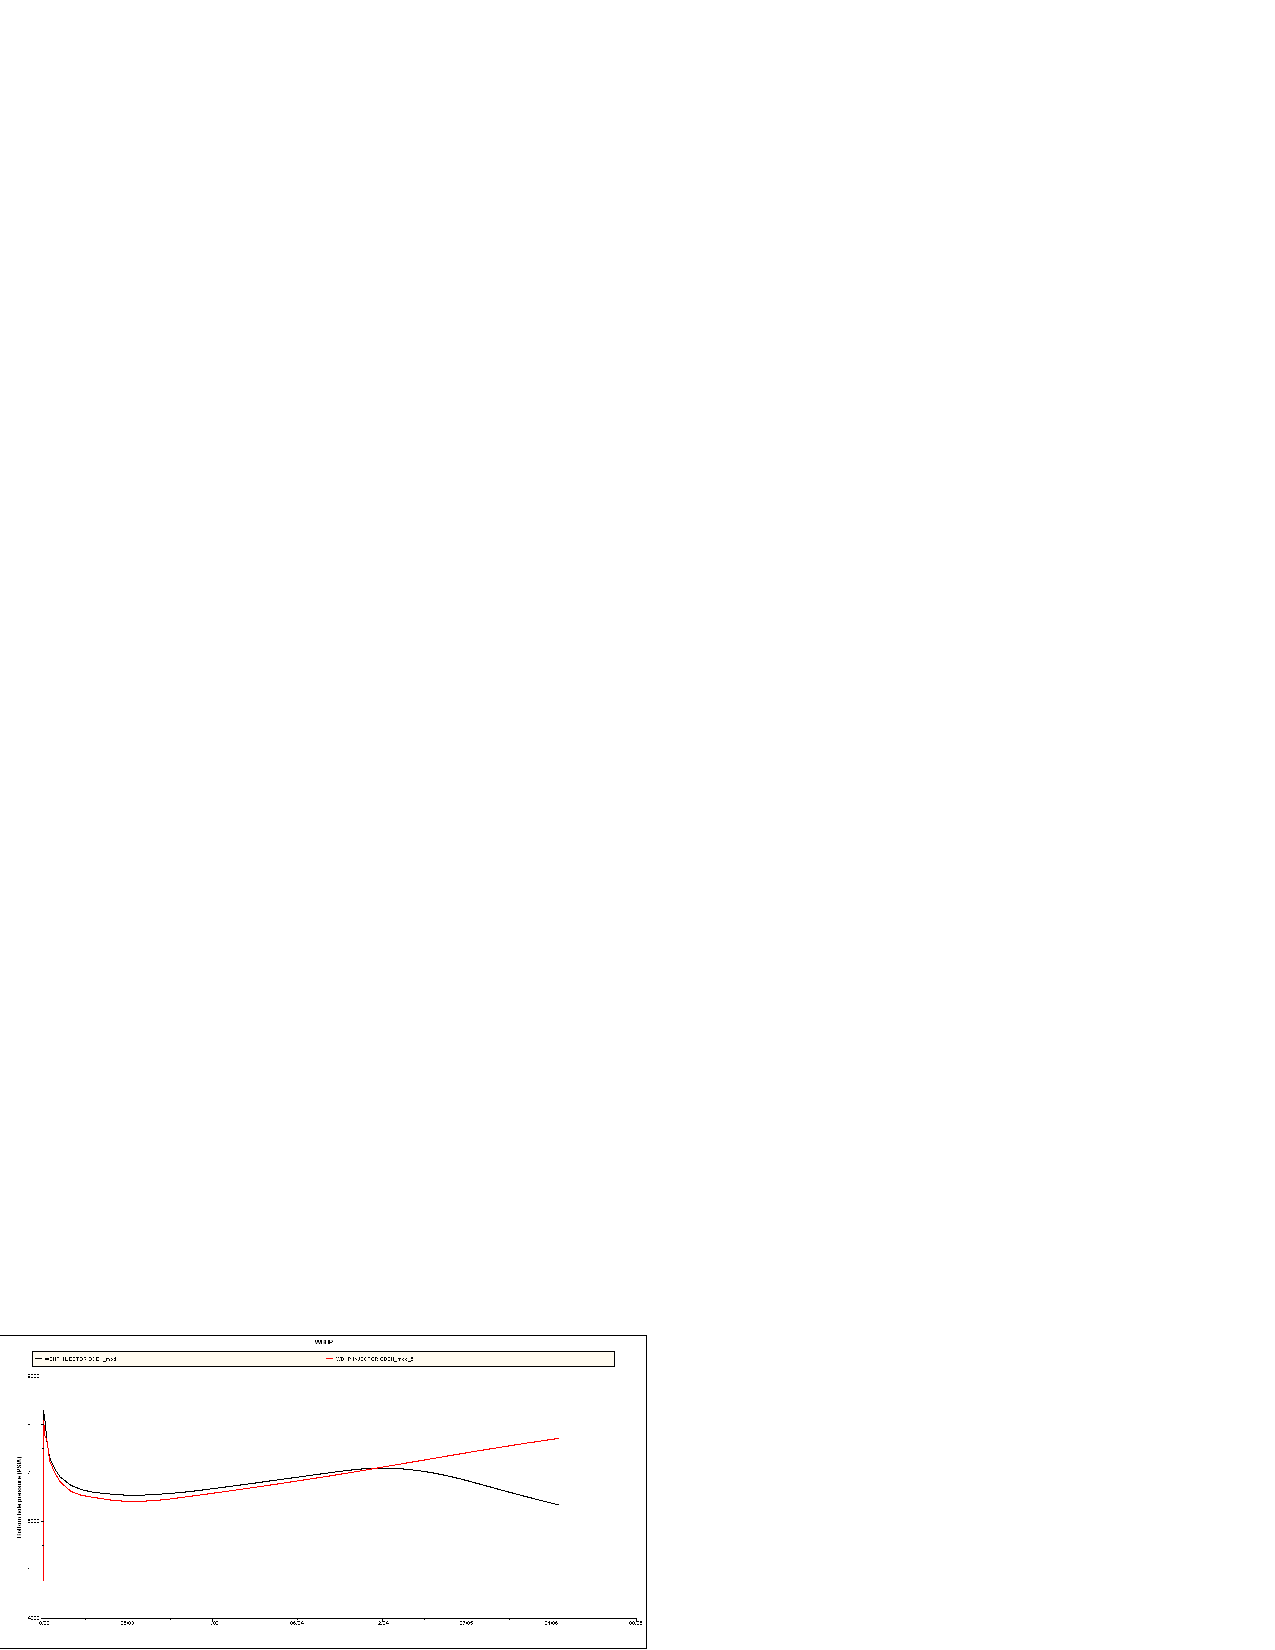
\includegraphics[clip=true, trim=0cm 0cm 10.6cm 22.6cm,width=1.3\textwidth]{graphics/wbhp_inj_comb.pdf}}
\centerline{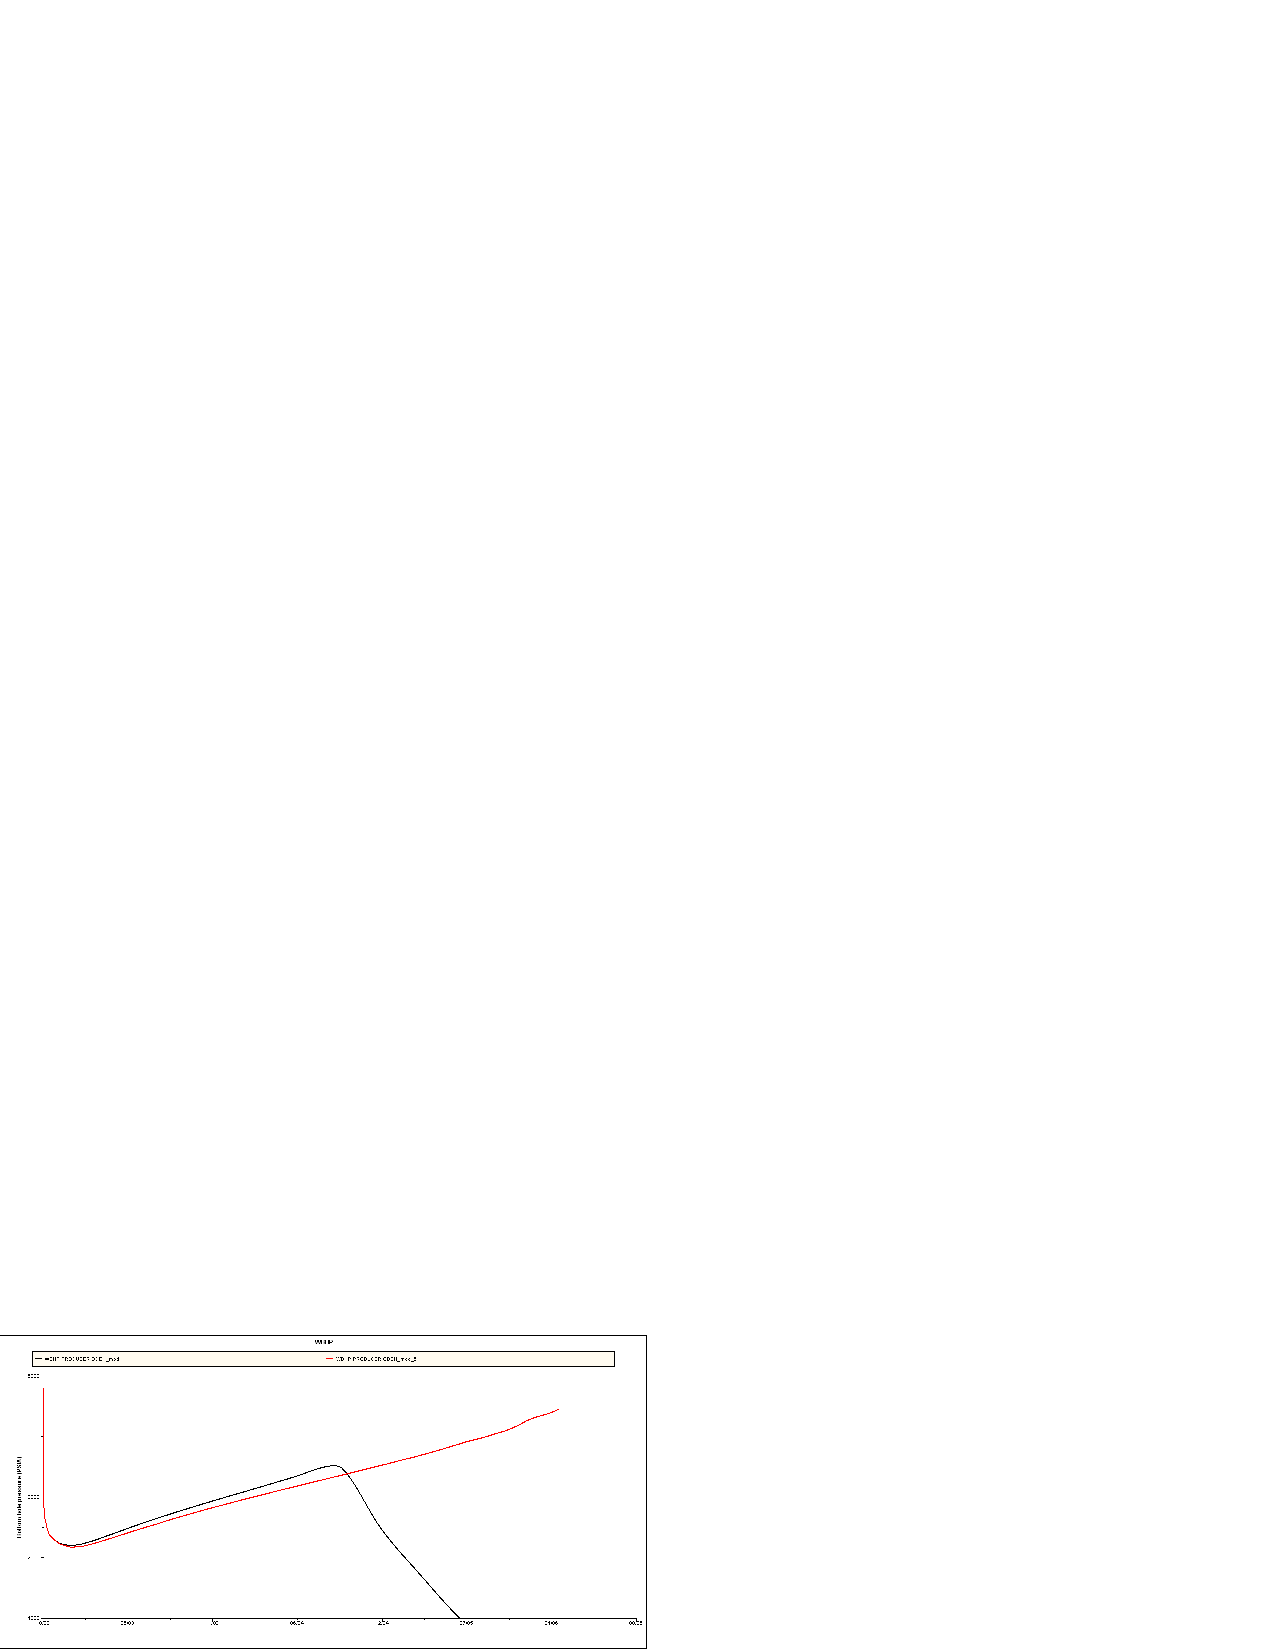
\includegraphics[clip=true, trim=0cm 0cm 10.6cm 22.6cm,width=1.3\textwidth]{graphics/wbhp_prod_comb.pdf}}
\centerline{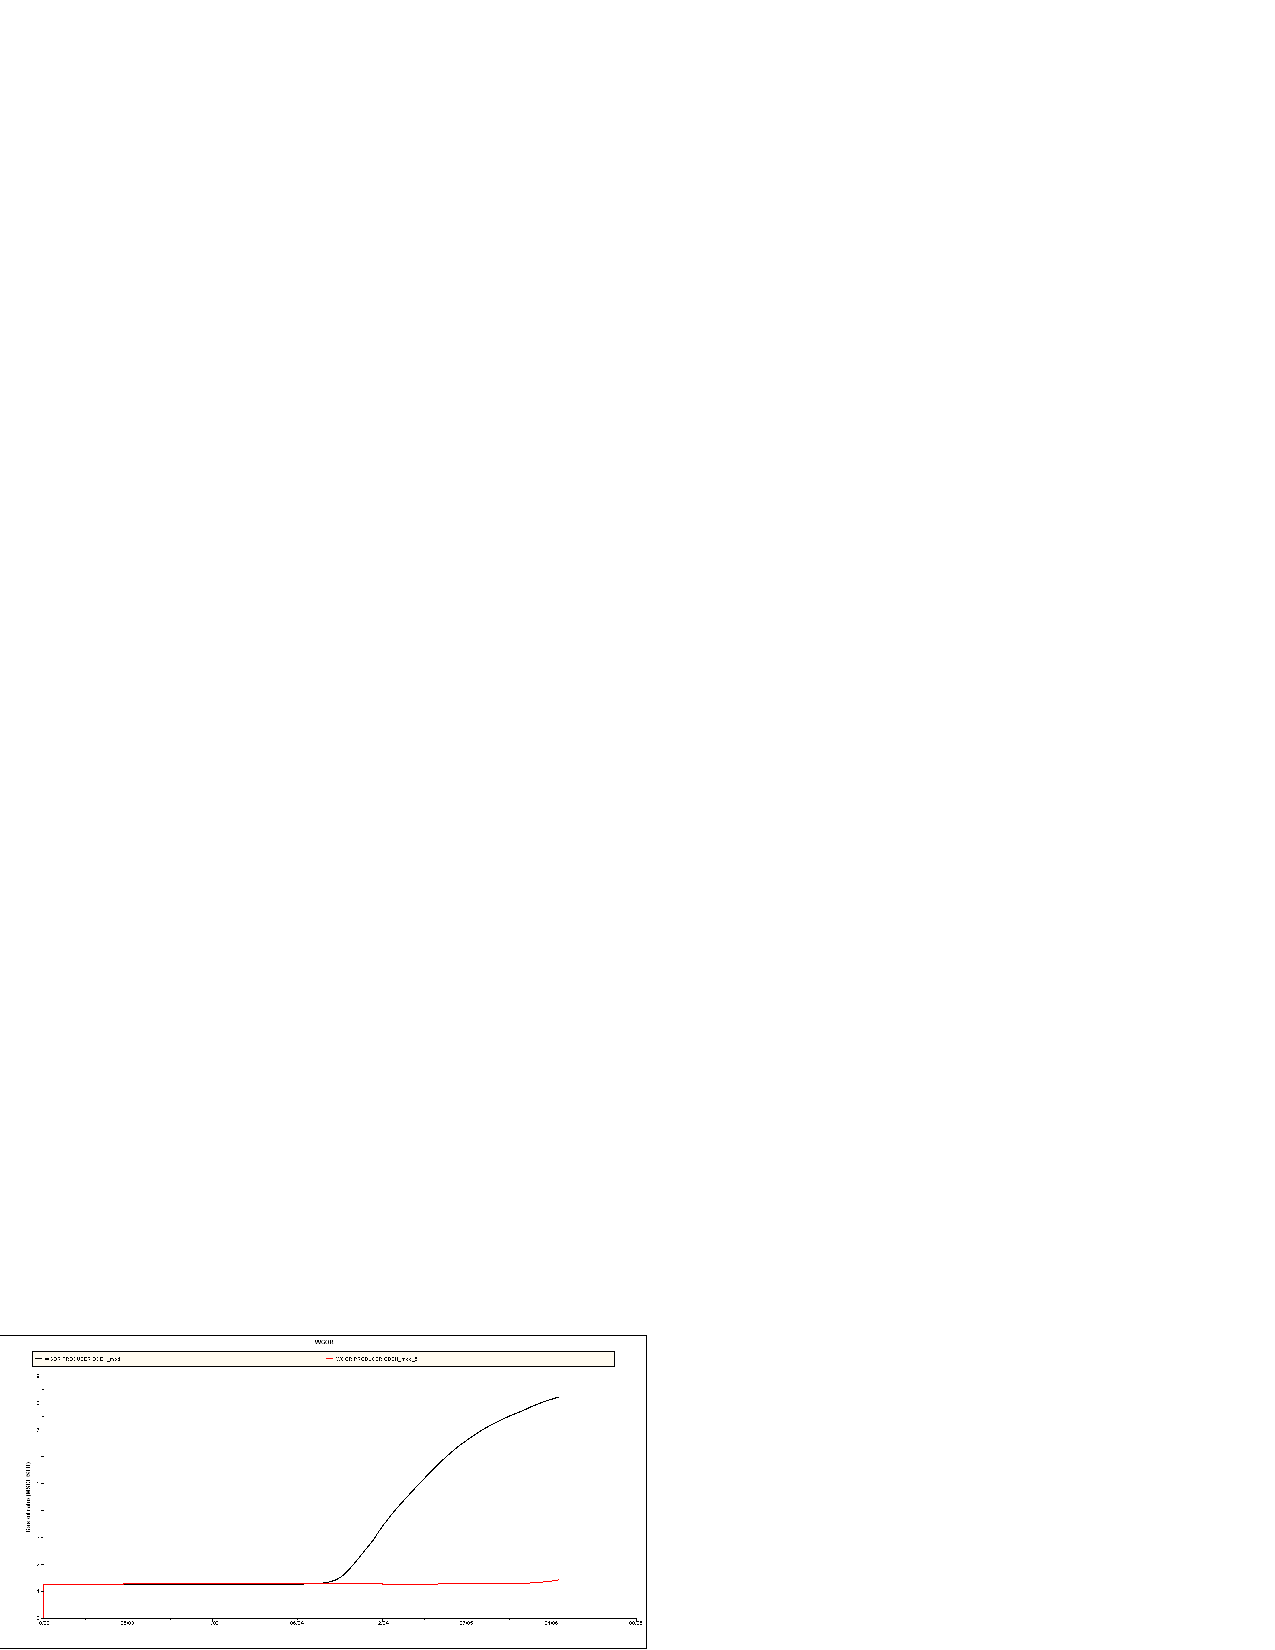
\includegraphics[clip=true, trim=0cm 0cm 10.6cm 22.6cm,width=1.3\textwidth]{graphics/wgor_comb.pdf}}

\centerline{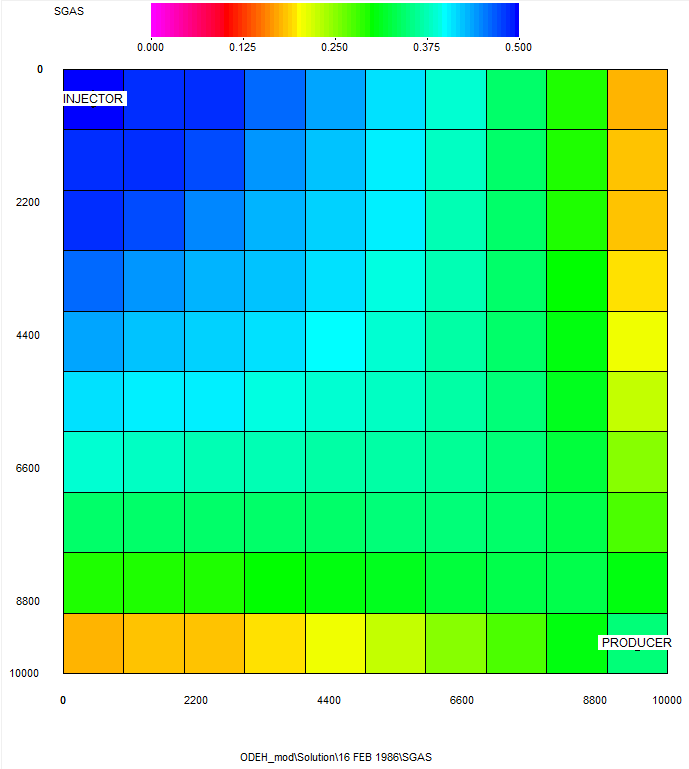
\includegraphics[width=0.8\textwidth]{graphics/grid_sgas_z1.PNG}}

\centerline{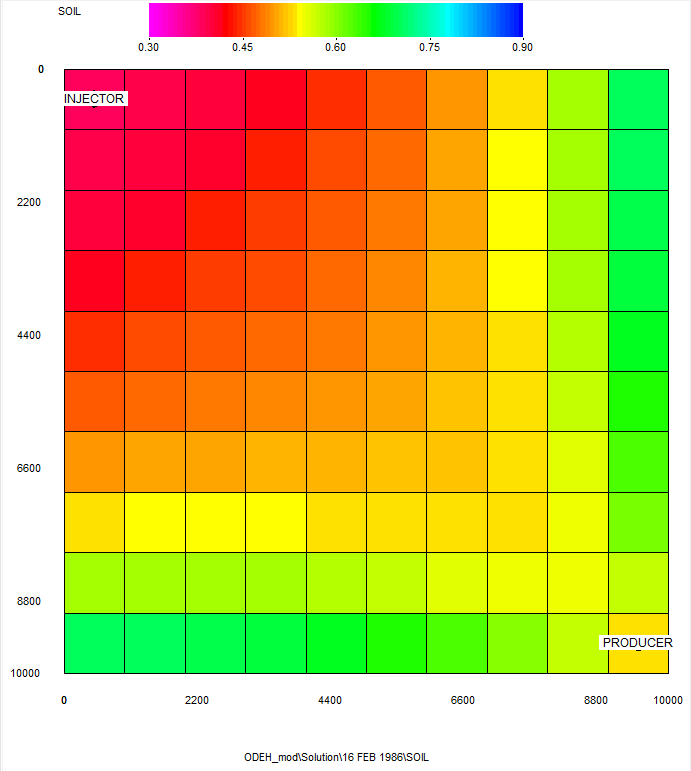
\includegraphics[width=0.8\textwidth]{graphics/grid_soil_z1.PNG}}

\centerline{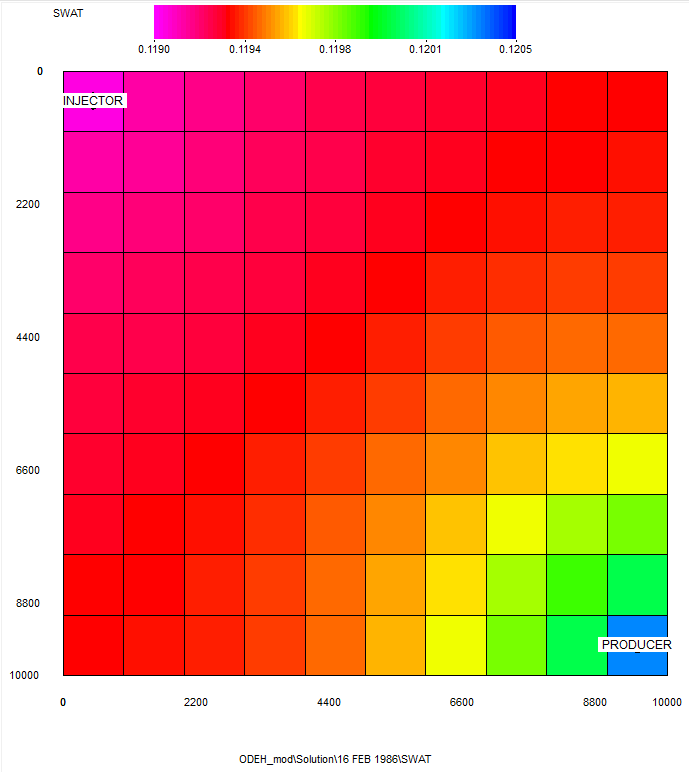
\includegraphics[width=0.8\textwidth]{graphics/grid_swat_z1.PNG}}




\end{document}
